\chapter{Étudiant}

\section{Présentation de l'interface}

  \subsection{Accueil etudiant: phase de voeux}
  \begin{figure}[H]
  	\centering
  	
  	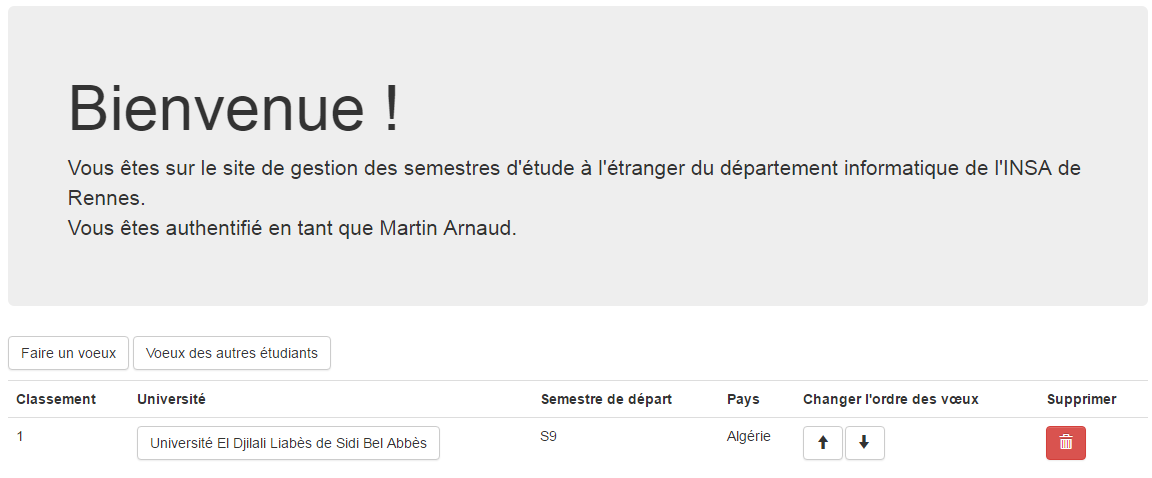
\includegraphics[width=16cm,height=9cm]{Images/Etudiant/faire_voeux_etud.png}
  	\caption{Accueil etudiant: phase de voeux}
  	\label{pv}
  \end{figure}


  \subsection{Accueil etudiant: phase dépôt de contrat d'étude}
  \begin{figure}[H]
  	\centering
  	
  	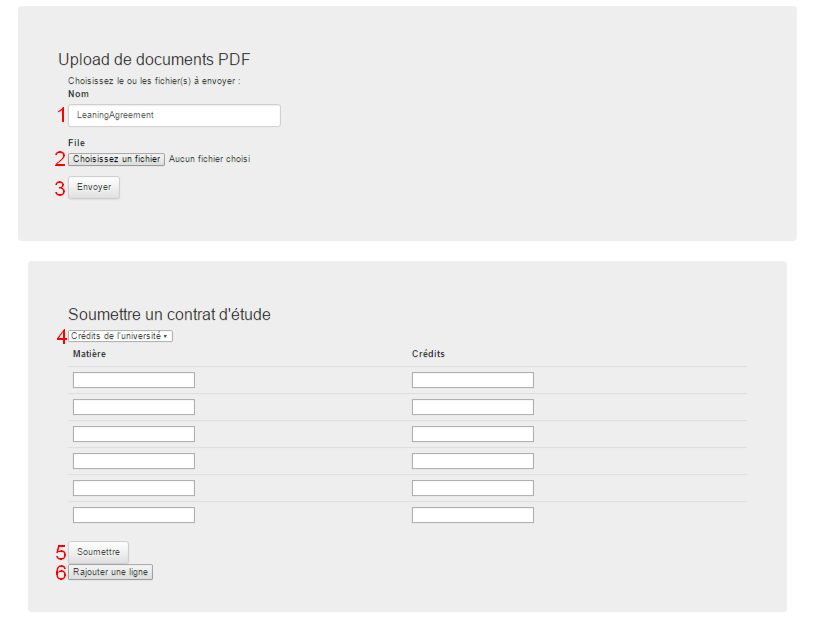
\includegraphics[width=16cm,height=9cm]{Images/Etudiant/learning_etud.png}
  	\caption{Accueil etudiant: phase dépôt de contrat d'étude}
  	\label{pl}
  \end{figure}


  \subsection{Accueil etudiant: phase de dépôt de notes}
  \begin{figure}[H]
  	\centering
  	
  	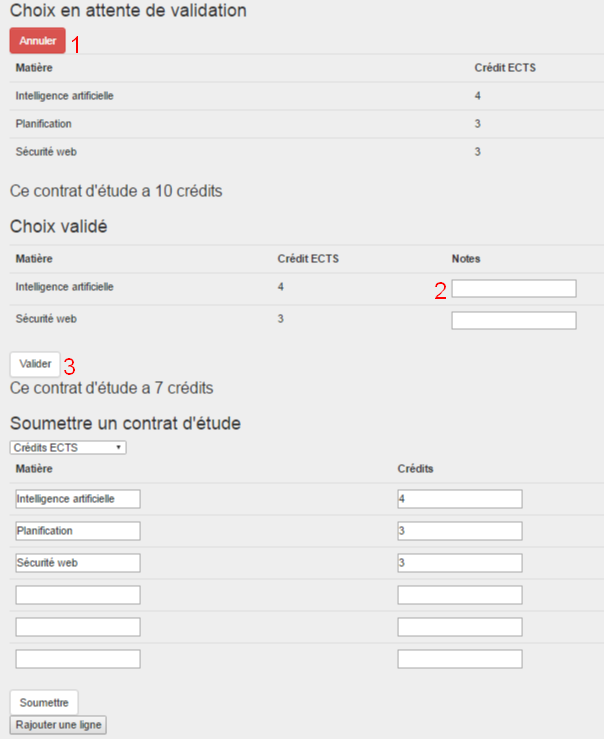
\includegraphics[width=14cm,height=12cm]{Images/Etudiant/notes_etud.png}
  	\caption{Accueil etudiant: phase de dépôt de notes}
  	\label{pn}
  \end{figure}



\section{Choix des destinations}

Depuis la page d'accueil, cliquez sur "Faire un vœux". Une fois sur la page "Liste des Universités", en face de l'université souhaitée, sélectionnez le type de mobilité que vous voulez dans le menu déroulant puis cliquez sur "Add" pour l'ajouter à votre liste de vœux.   
 
\section{Gestion des vœux}

Depuis la page d'accueil, grâce aux bouton à droite de vos vœux, vous pouvez modifier l'ordre de vos vœux ou en supprimer.

\section{Proposition de contrat d'étude}

Depuis la page d'accueil, dans la section "Soumettre un contrat d'étude", sélectionner le type de crédit ayant cours dans votre université d'accueil puis entrez le nom des matières et le nombre de crédits rapportés par la matière.
Il est ensuite possible, en répétant la même manipulation, de soumettre d'autres contrats d'études.

\section{Dépôt de fichiers}

Depuis la page d'accueil, dans la section "Upload de documents", vous pouvez ajouter des fichiers pour l'élève en question. Pour cela, entrez le nom souhaité pour le document puis cliquer sur "choisissez un fichier" et sélectionnez le fichier. Cliquez enfin sur "envoyer" 

\section{Dépôt de notes}